% %%%%%%%%%%%%%%%%%%%%%%%%%%%%%%%%%%%%%%%%%%%%%%%%%%%%%%%%%%%%%%%%%%%%%%
% %%%%%%%%%%%%%%%%%%%%%%%%%%%%%%%%%%%%%%%%%%%%%%%%%%%%%%%%%%%%%%%%%%%%%%
% %%%%                   Auxiliary units
% %%%%%%%%%%%%%%%%%%%%%%%%%%%%%%%%%%%%%%%%%%%%%%%%%%%%%%%%%%%%%%%%%%%%%%
% %%%%%%%%%%%%%%%%%%%%%%%%%%%%%%%%%%%%%%%%%%%%%%%%%%%%%%%%%%%%%%%%%%%%%%

\section{Auxiliary units}\label{sec:aux}

\glyph{Auxiliary units} are decorations used on \glyph{entities} (\sect{entity}) and \glyph{interactions} (\sect{interaction}) to further refine their semantics.  \SBGNERLone{} provides two \glyph{auxiliary units}, the \glyph{unit of information} and the \glyph{state variable}.

%%%%%%%%%%%%%%%%%%%%%%%%%%%%%%%%%%%%%%%%%%%%%%%%%%%%%%%%%%%%%%%%%%%%%%
%%                     Unit of Information
%%%%%%%%%%%%%%%%%%%%%%%%%%%%%%%%%%%%%%%%%%%%%%%%%%%%%%%%%%%%%%%%%%%%%%
\color{blue}

\subsection{Glyph: \glyph{Unit of information}}
\label{sec:unitInformation}

When representing biological entities, it is often necessary to convey some abstract information about the entity's function or structure.  The SBGN \glyph{unit of information} is a decoration that can be used in this situation to add information to a glyph.  Some example uses of a \glyph{unit of information} include (but are not limited to) providing an identifier for an interaction, characterizing a logical part of an entity, information about the physical environment, or the specific type of biological entity it is decorating.

\begin{glyphDescription}

\glyphSboTerm Not applicable.

\glyphContainer A unit of information is represented by a rectangle.  The long side of the rectangle should be oriented parallel to the border of the \glyph{entity} being annotated by the \glyph{unit of information}. The center of the bounding box of a \glyph{state of information} should be located on the mid-line of the border of the \glyph{entity}.

\glyphLabel A \glyph{unit of information} is identified by a label placed in an unbordered box containing a string of characters.  The characters can be distributed on several lines to improve readability, although this is not mandatory.  The label box must be attached to the center of the container.  The label may spill outside of the container.

The label defines the information carried by the \glyph{unit of information}.  For certain predefined types of information having controlled vocabularies associated with them, SBGN defines specific prefixes that must be included in the label to indicate the type of information in question.  The controlled vocabularies predefined in \SBGNERLone are described in \sect{CVs} and summarized in the following list:

\begin{center}
  \begin{itemize}\setlength{\parskip}{0ex}
  \item[\texttt{mt}] entity material type
  \item[\texttt{ct}] entity conceptual type
  \end{itemize}
\end{center}

\glyphAux A \glyph{unit of information} does not carry any auxiliary items.

\end{glyphDescription}

\begin{figure}[H]
  \centering
  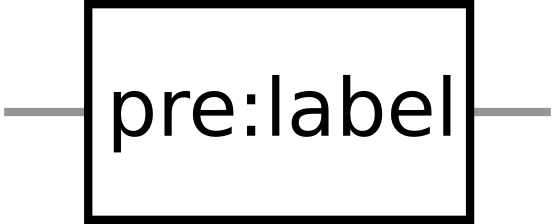
\includegraphics[scale = 0.3]{images/unitInformation}
  \caption{The \ER glyph for \glyph{unit of information}.}
  \label{fig:unitInformation}
\end{figure}

\begin{figure}[H]
  \centering
  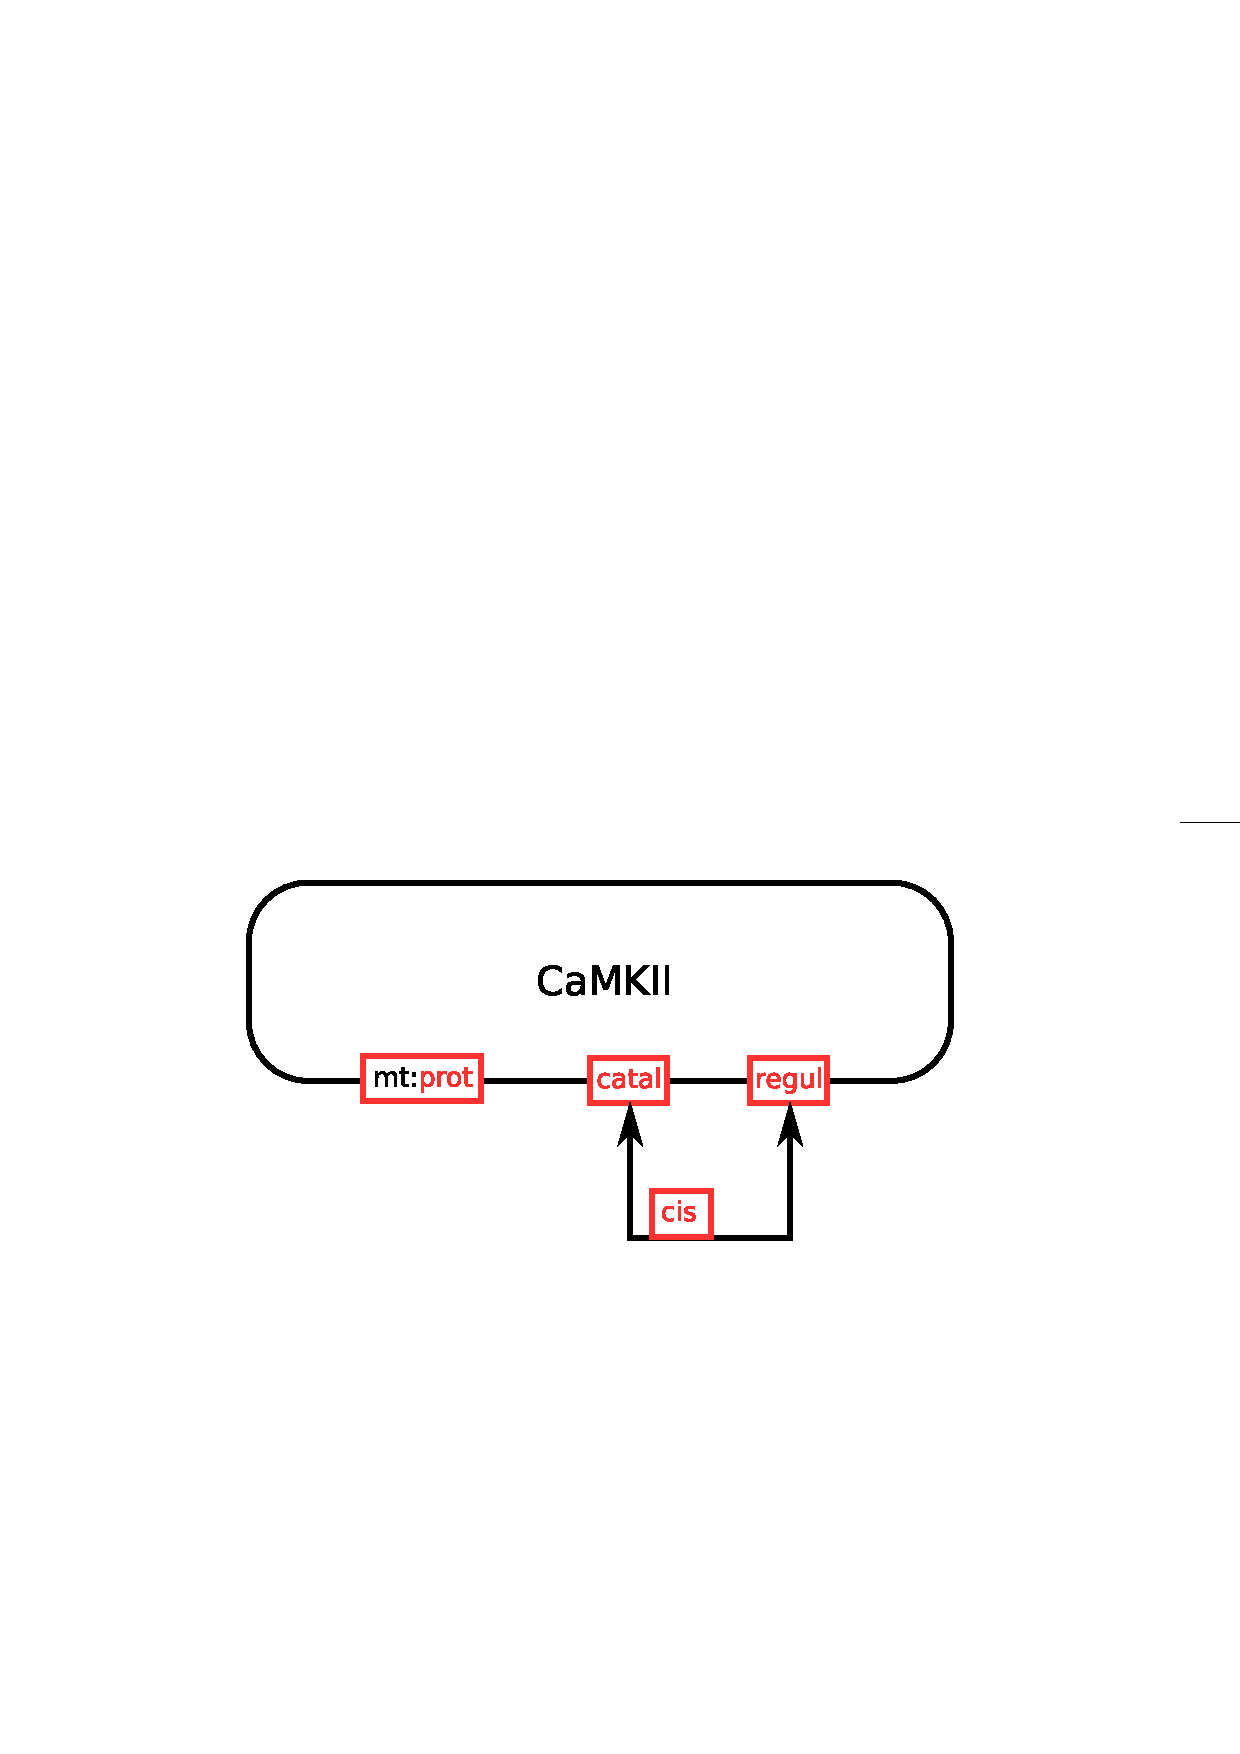
\includegraphics[scale = 0.5]{examples/ex-unitInformation}
  \caption{Using a \glyph{unit of information} to represent the fact that the entity ``CaMKII'' is a protein.}
  \label{fig:ex-unitInformation}
\end{figure}

\normalcolor

%%%%%%%%%%%%%%%%%%%%%%%%%%%%%%%%%%%%%%%%%%%%%%%%%%%%%%%%%%%%%%%%%%%%%%
%%                     State variable
%%%%%%%%%%%%%%%%%%%%%%%%%%%%%%%%%%%%%%%%%%%%%%%%%%%%%%%%%%%%%%%%%%%%%%
%\color{blue}

\subsection{Glyph: \glyph{State variable}}
\label{sec:stateVariable}

Many biological entities such as molecules can exist in different \emph{states}, meaning different physical or informational configurations.  These states can arise for a variety of reasons.  For example, macromolecules can be subject to post-synthesis modifications, wherein residues of the macromolecules (amino acids, nucleosides, or glucid residues) are modified through covalent linkage to other chemicals.  Other examples of states are alternative conformations as in the closed/open/desensitized conformations of a transmembrane channel, and the active/inactive forms of an enzyme.

SBGN provides a means of associating one or more \glyph{state variables} with an entity; each such variable can be used to represent a dimension along which the state of the overall entity can vary.  When an entity can exist in different states, the state of the instance of the entity % (\ie the SBGN object) 
can be described by the current values of all its \glyph{state variables}, and the values of the \glyph{state variables} of all its possible components, recursively.

In \SBGNERLone, \glyph{state variables} are also used to describe the localisation in compartments (a transport is therefore described as a state variable assignment, see \sect{assignment}).

\begin{glyphDescription}

\glyphSboTerm Not applicable.

\glyphContainer A \glyph{state variable} is represented by a ''stadium'' container, that is two semicircles of same radius joined by parallel segments, as shown in \fig{state-var}.  The parallel segment axis should be tangent to the border of the glyph of the \glyph{entity} being modified by the \glyph{state variable}. The center of the bounding box of a \glyph{state variable} should be located on the mid-line of the border of the \glyph{entity}.

\glyphLabel A \glyph{state variable} is identified by a label placed in an unbordered box containing a string of characters.  The characters can be distributed on several lines to improve readability, although this is not mandatory.  The label box must be attached to the center of the container.  The label may spill outside of the container.

\glyphAux A \glyph{state variable} does not carry any auxiliary items.  

\end{glyphDescription}

\begin{figure}[H]
  \centering
  \includegraphics[scale = 0.3]{images/stateVariable}
  \caption{The \ER glyph for \glyph{state variable}. From left to right, horizontal \glyph{state variable}, vertical \glyph{state variable}, \glyph{location}, \glyph{existence}.}
  \label{fig:state-var}
\end{figure}

Two state variables are predefined. The variable \glyph{existence} is used to represent the creation or destruction of entities, as seen on \fig{ex-existence}\label{sec:existence}. \glyph{Existence} can take two values, true (T) or false (F). The variable is represented by a circle vertically divided in two. One hemicircle is black, and the other white. 

\begin{figure}[H]
  \centering
  \includegraphics[scale = 0.5]{examples/ex-existence}
  \caption{Using the \glyph{state variable} \glyph{existence} to represent the appearance of calcium following a depolarisation.}
  \label{fig:ex-existence}
\end{figure}

The variable \glyph{location} is used to represent the physical location of an entity, as seen on \fig{ex-location}\label{sec:location}. \glyph{Location} can take any value, but there can be only one \glyph{location} per instance of an entity. The variable is represented by a circle containing two perpendicular segments, an abstract version of the usual slanted pin.

\begin{figure}[H]
  \centering
  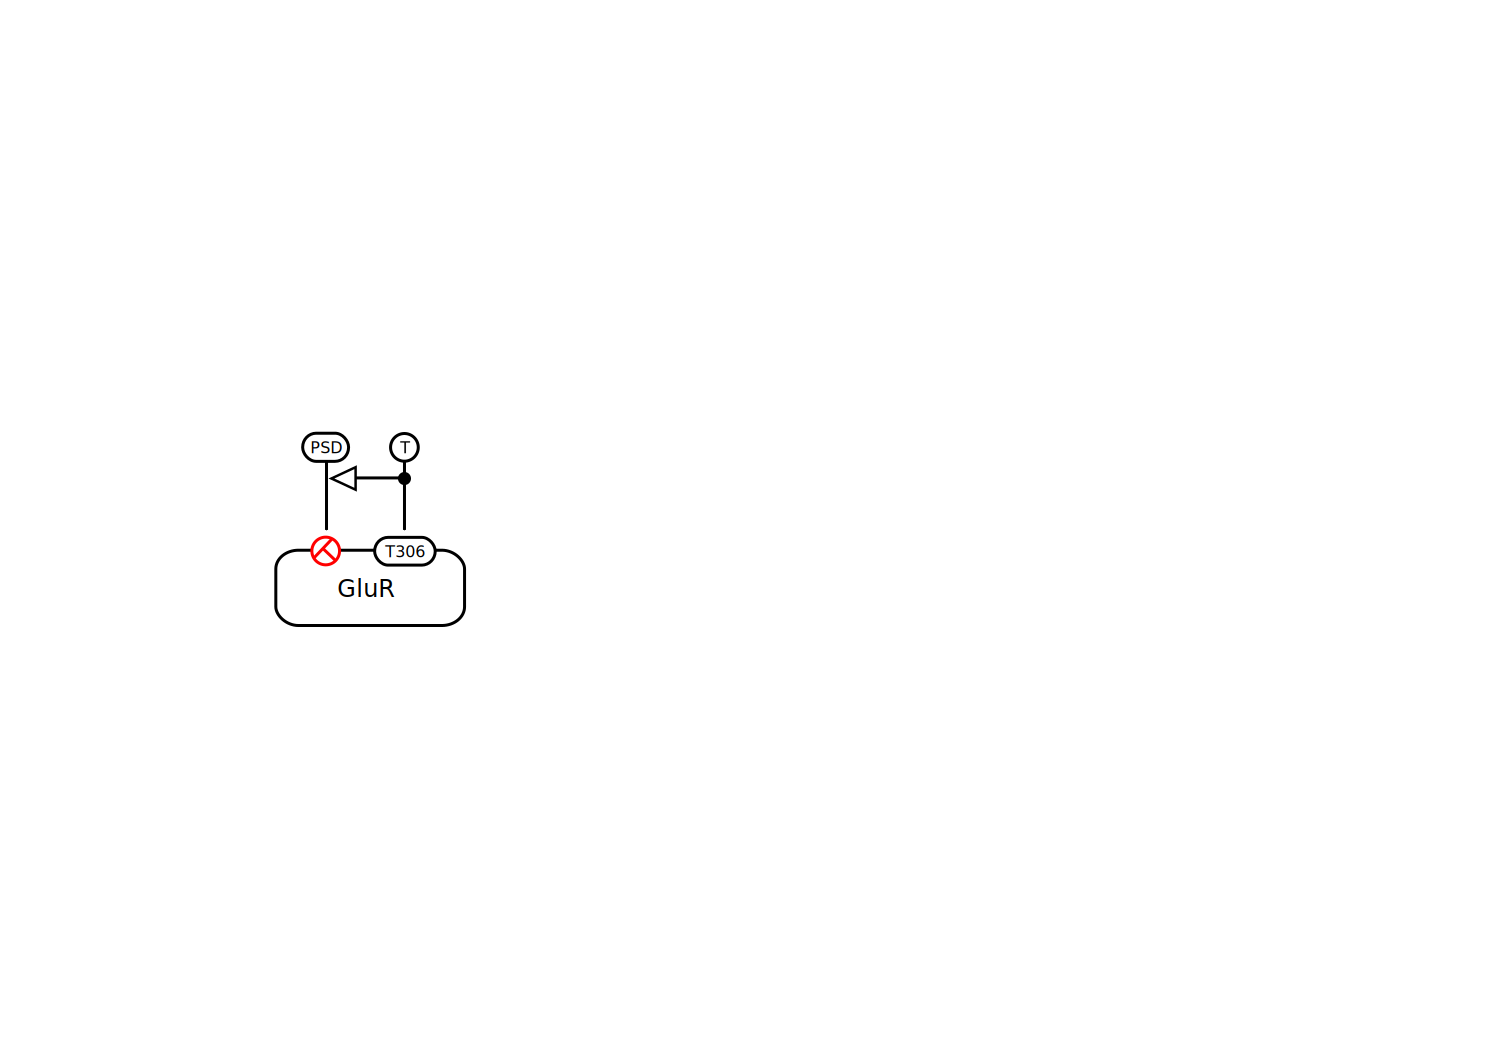
\includegraphics[scale = 0.5]{examples/ex-location-2}
  \caption{Using the \glyph{state variable} \glyph{location} to represent the fact that phosphorylation of glutamate receptors stimulate their incorporation in the post-synaptic density.}
  \label{fig:ex-location}
\end{figure}

%\normalcolor

% The following is for [X]Emacs users.  Please leave in place.
% Local Variables:
% TeX-master: "../sbgn_ER-level1"
% End:


%%%%%%%%%%%%%%%%%%%%%%%%%%%%%%%%%%%%%%%%%%%%%%%%%%%%%%%%%%%%%%%%%%%%%%
%%                     Variable value
%%%%%%%%%%%%%%%%%%%%%%%%%%%%%%%%%%%%%%%%%%%%%%%%%%%%%%%%%%%%%%%%%%%%%%
%\color{blue}

\subsection{Glyph: \glyph{Variable value}}
\label{sec:variableValue}

\begin{glyphDescription}
 
\glyphSboTerm Not applicable.
 
\glyphContainer A \glyph{variable value} is represented by a ''stadium'' container, that is two hemicercles of same radius joined by parallel segments, as shown in \fig{var-value}. 
 
\glyphLabel A \glyph{variable value} is identified by a label placed in an unbordered box containing a string of characters.  The characters can be distributed on several lines to improve readability, although this is not mandatory.  The label box must be attached to the center of the container.  The label may spill outside of the container.

\glyphAux A \glyph{state variable} does not carry any auxiliary items.  
 
\end{glyphDescription}
 
\begin{figure}[H]
   \centering
   \includegraphics[scale = 0.3]{images/variableValue}
   \caption{The \ER glyph for \glyph{state variable}. From left to right, horizontal state variable, vertical state variable, \glyph{Location}, \glyph{existence}.}
   \label{fig:var-value}
\end{figure}

A \glyph{variable value} is linked to a \glyph{state variable} (see \sect{stateVariable}) through \glyph{assignment} (see \sect{assignment}). 

A \glyph{state variable} does not necessarily have to be Boolean-valued.  For example, an ion channel can possess several conductance states; a receptor can be inactive, active and desensitized; and so on.  As another example, a \glyph{state variable} ``ubiquitin'' could also carry numerical values corresponding to the number of ubiquitin molecules present in the tail.

\begin{figure}[H]
  \centering
  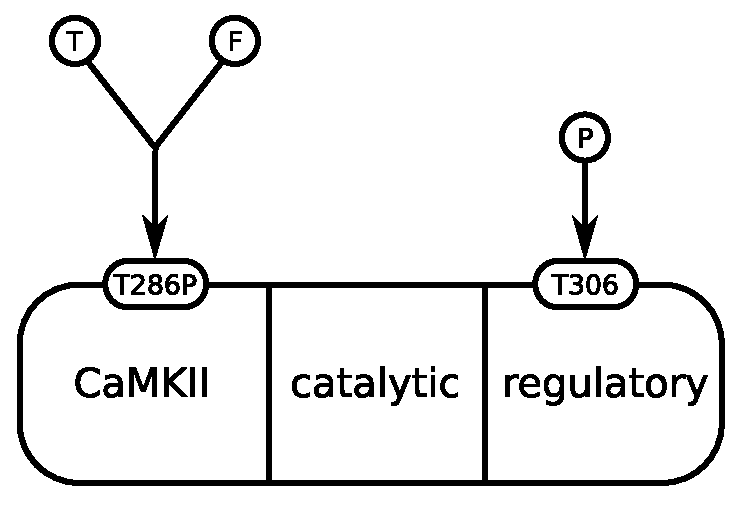
\includegraphics[scale = 0.5]{examples/ex-stateVariable}
  \caption{Two examples of \glyph{state variables} used to represent phophorylation of a threonine residue. While only the value ``phosphorylated'' is assigned to T306, the variable T286P can take the values true or false, which allow for representing dephosphorylation as well as phosphorylation.}
  \label{fig:ex-state-Variable}
\end{figure}

Two state variables are predefined. The variable \glyph{existence} is used to represent the creation or destruction of entities, as seen on \fig{ex-existence}\label{sec:existence}. \glyph{Existence} can take two values, true (T) or false (F). The variable is represented by a circle vertically divided in two. One hemicircle is black, and the other white. 

\begin{figure}[H]
  \centering
  \includegraphics[scale = 0.5]{examples/ex-existence}
  \caption{Using the \glyph{state variable} \glyph{existence} to represent the appearance of calcium following a depolarisation.}
  \label{fig:ex-existence}
\end{figure}

The variable \glyph{location} is used to represent the physical location of an entity, as seen on \fig{ex-location}\label{sec:location}. \glyph{Location} can take any value, but there can be only one \glyph{location} per entity. The variable is represented by a circle containing two perpendicular segments, an abstract version of the usual slanted pin.

\begin{figure}[H]
  \centering
  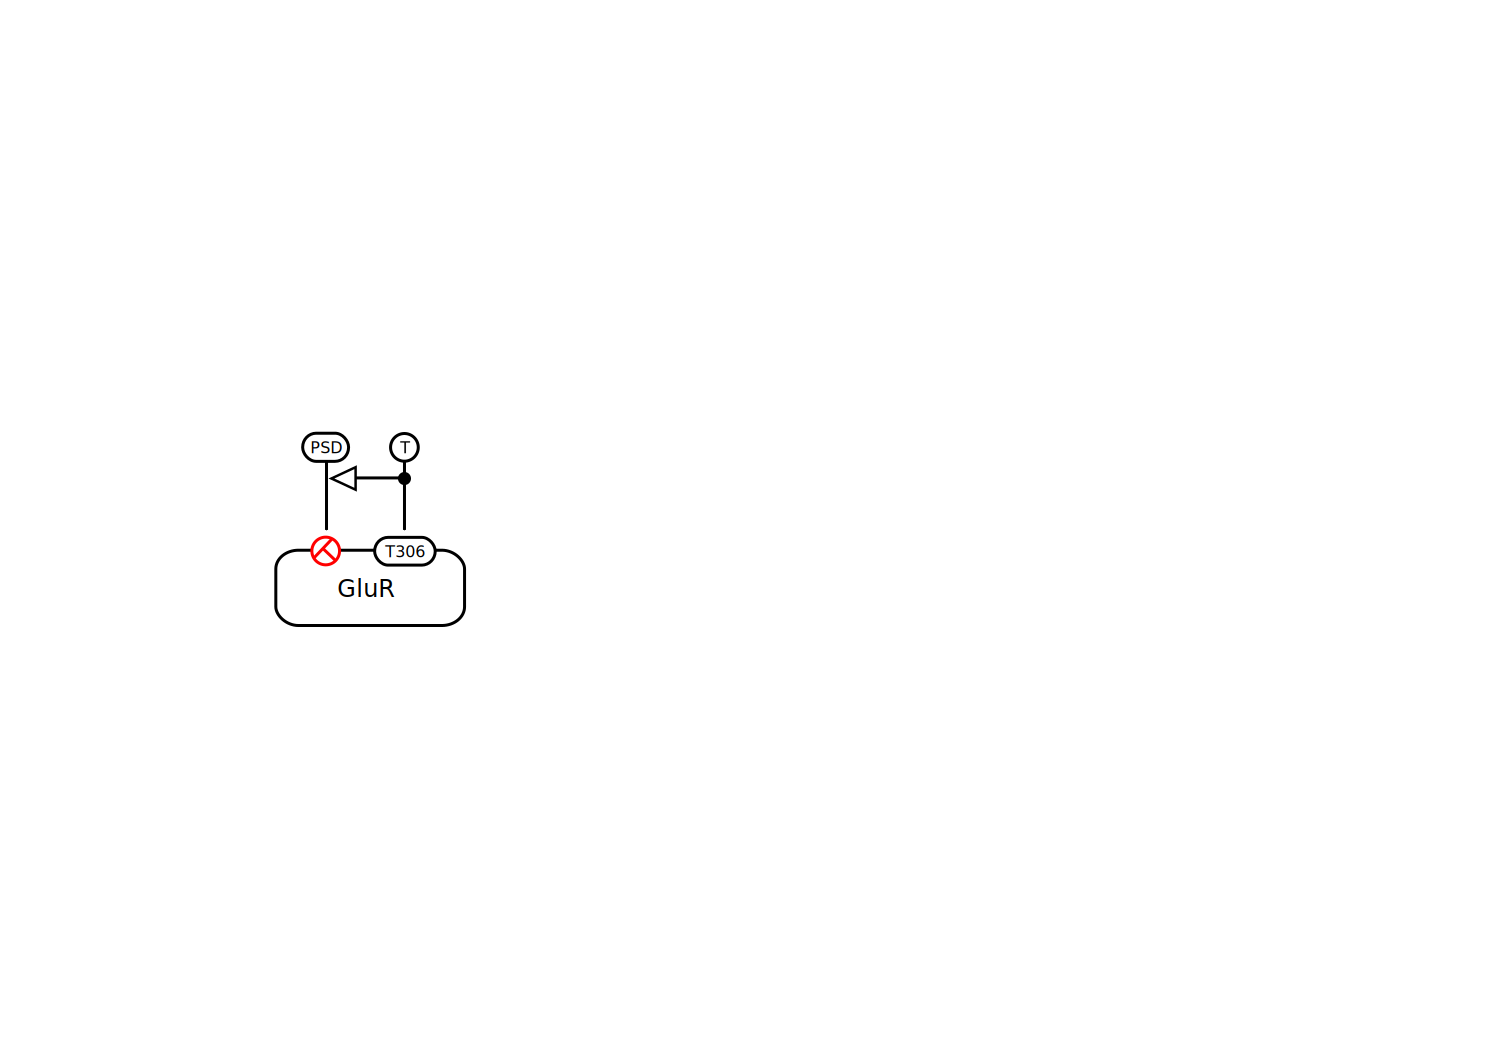
\includegraphics[scale = 0.5]{examples/ex-location-2}
  \caption{Using the \glyph{state variable} \glyph{location} to represent the fact that phosphorylation of glutamate receptors stimulate their incorporation in the post-synaptic density.}
  \label{fig:ex-location}
\end{figure}


% \begin{figure}[H]
%   \centering
%   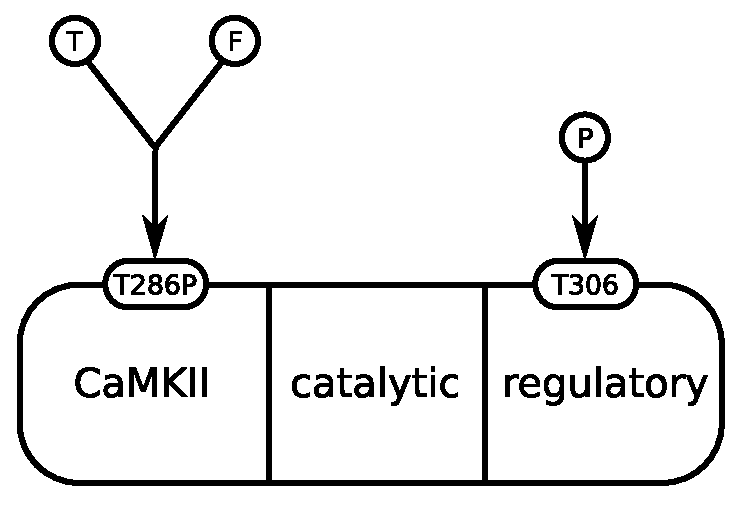
\includegraphics[scale = 0.5]{examples/ex-stateVariable}
%   \caption{Two examples of \glyph{state variables} used to represent phophorylation of a threonine residue. While only the value ``phosphorylated'' is assigned to T306, the variable T286P can take the values true or false, which allow for representing dephosphorylation as well as phosphorylation.}
%   \label{fig:ex-state-Variable}
% \end{figure}
% 
% Two state variables are predefined. The variable \glyph{existence} is used to represent the creation or destruction of entities, as seen on \fig{ex-existence}\label{sec:existence}. \glyph{Existence} can take two values, true (T) or false (F). The variable is represented by a circle vertically divided in two. One hemicircle is black, and the other white. 
% 
% \begin{figure}[H]
%   \centering
%   \includegraphics[scale = 0.5]{examples/ex-existence}
%   \caption{Using the \glyph{state variable} \glyph{existence} to represent the appearance of calcium following a depolarisation.}
%   \label{fig:ex-existence}
% \end{figure}
% 
% The variable \glyph{location} is used to represent the physical location of an entity, as seen on \fig{ex-location}\label{sec:location}. \glyph{Location} can take any value, but there can be only one \glyph{location} per entity. The variable is represented by a circle containing two perpendicular segments, an abstract version of the usual slanted pin.
% 
% \begin{figure}[H]
%   \centering
%   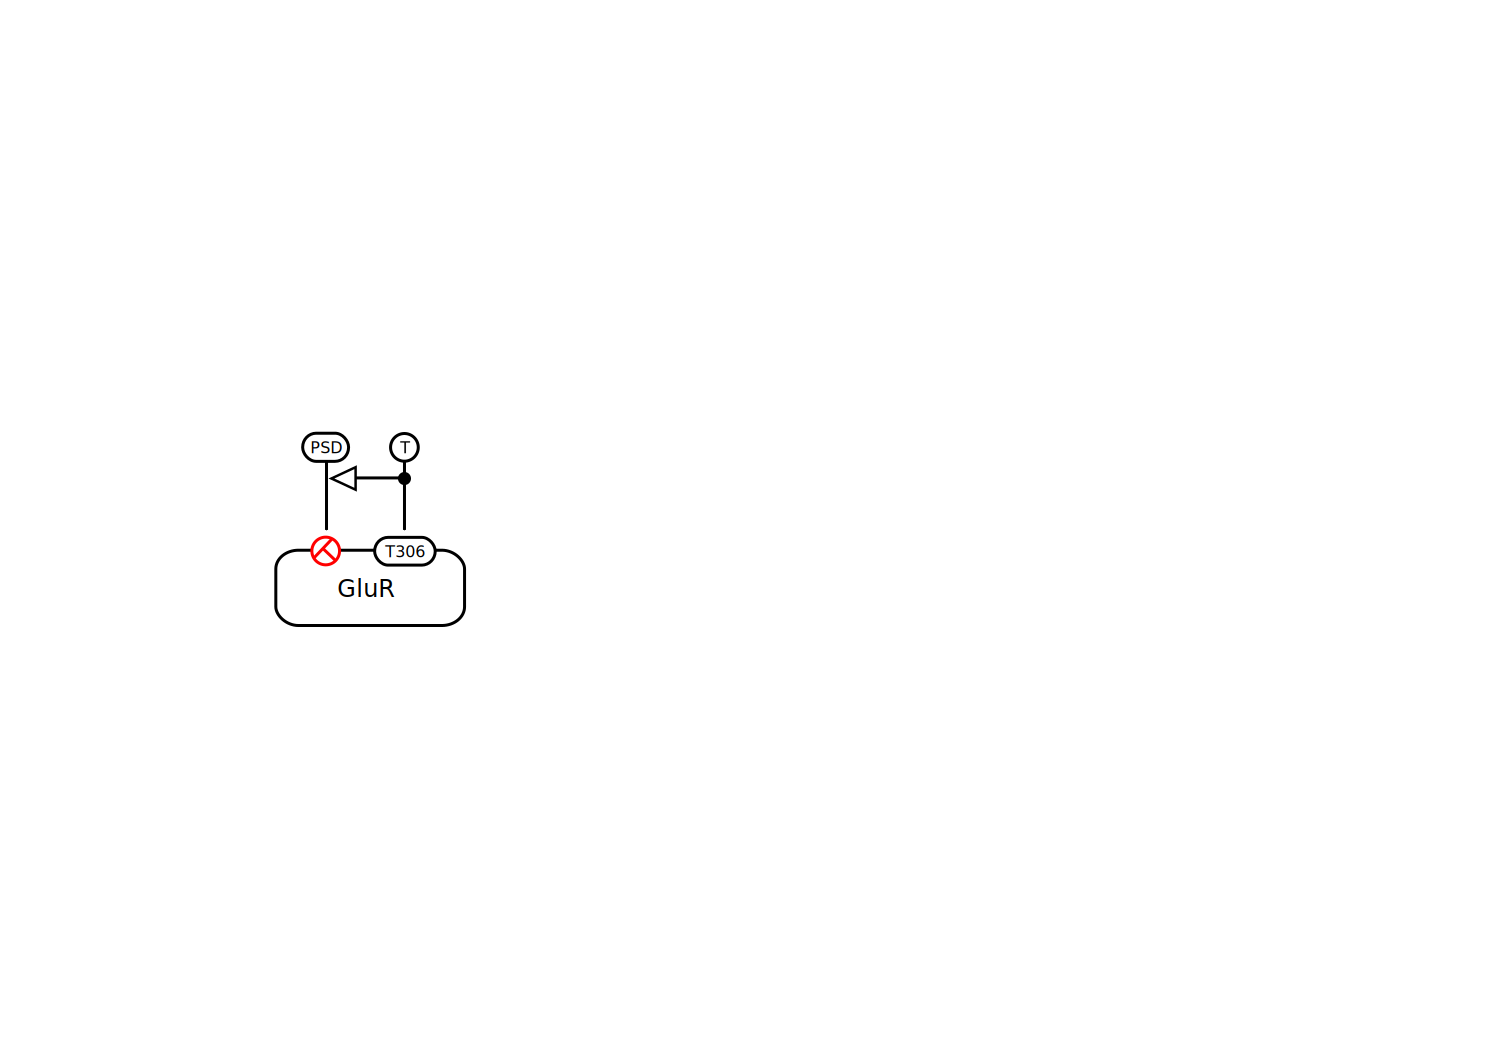
\includegraphics[scale = 0.5]{examples/ex-location-2}
%   \caption{Using the \glyph{state variable} \glyph{location} to represent the fact that phosphorylation of glutamate receptors stimulate their incorporation in the post-synaptic density.}
%   \label{fig:ex-location}
% \end{figure}

%\normalcolor

% The following is for [X]Emacs users.  Please leave in place.
% Local Variables:
% TeX-master: "../sbgn_ER-level1"
% End:

